\chapter{Detailed Design}

Detailed design done by specifying algorithm and structure that makes up the interior modules. Usually there are many choice but from the different alternatives available. The one, which offer greatest efficiency, simply functionality is selected based on the relative important of these criteria.

\section{Data Dictionary}
A data dictionary provides a complete documentation of all the element of system like data items, data stores(database) and data flow. Data described in data dictionary carries the details of the type, data name, database name, data description and characterization. Data Dictionary covers the whole organization or a database. Data Dictionary is only collection of the element definition. Entries in a data dictionary include the name of the data item and attributes. Data Dictionary has been proposed a formal grammar for describing the contents of the definition of all data mentioned in the data flow diagram. In process specification, composite data is defined in terms of the meaning each of the values that it can assume.

\section{Input and output Design}

The goal of input key is to input data as accurately as possible. Here inputs are designed effectively so that the error made by operation is minimized. The input to the system has been designed and coordination in such way that there format is similar in all forms. Forms are designed in such way that relevant information is
grouped together and they are placed on a single frame, so as to access easily. At the time of data entry the verification and validation of the data were done. Input key is the most part of the overall system design, which requires very careful attention.
Often the collection of the input data is most expensive part of the system. Many errors may occur during the phase of the design. So to make the system study, the inputs given by the user is strictly validated before making a manipulation with it.
\\
\\
The output key is another very important phase. The outputs are mainly used to communicate with the user, processing the input data given by the user. It is documented in each stage of the project to ensure free output. The output screens are designed in very simple and easy to understand format. The quality, urgency and the frequency of outputs should be taken into consideration. All user option is presented in well-formatted forms. The quality refers to the way by which the output is presented to the user. The reports can be used for day-to-day functioning of the business as well as management information. The reports, if generated with the specific report criteria and in a timely manner, help in operational efficiency, detecting and minimizing of errors as well as provide the pointers towards control weakness.		
		
		% This section type your project contents 
		
		
\pagebreak
\subsection{Login Form}
\textbf{login}
\begin{center}
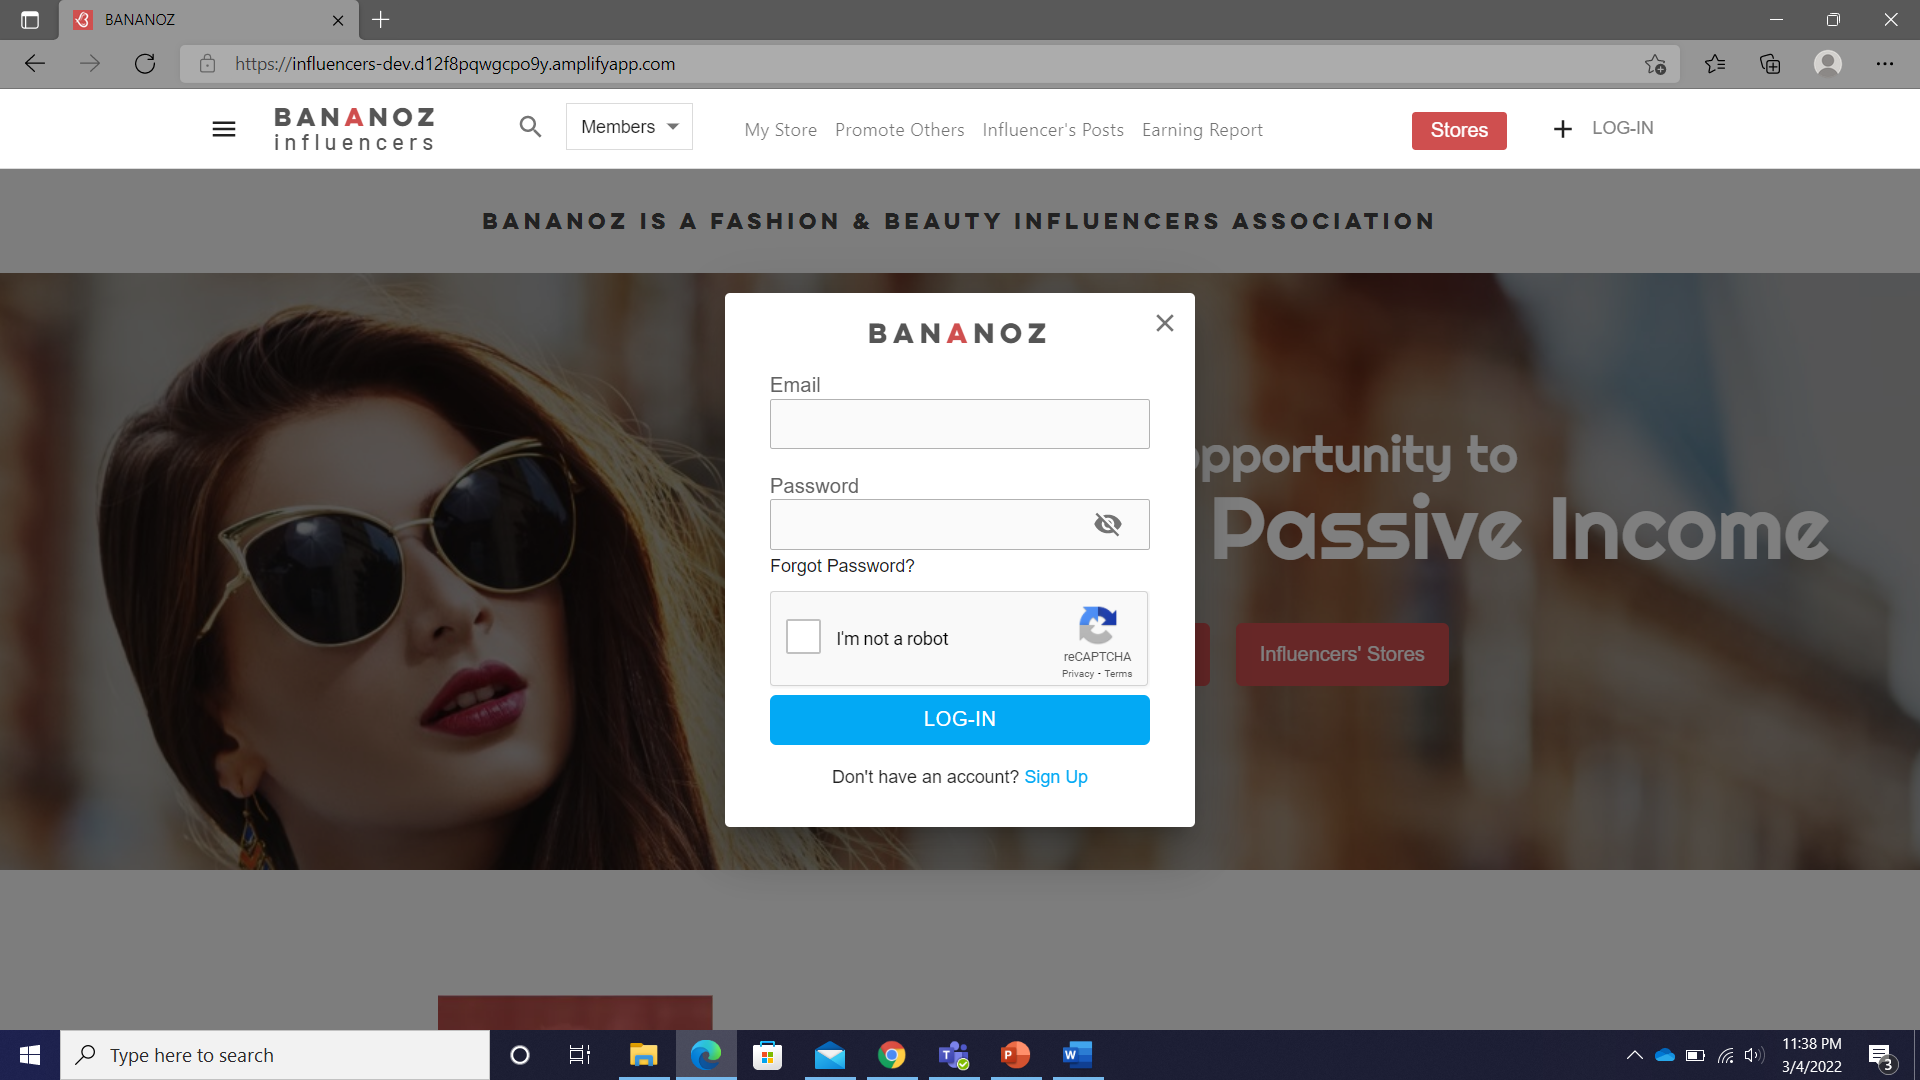
\includegraphics[height=9cm,width=14cm]{Admin/user-login.png}
\end{center}

% This section type your project contents 
\textbf{My Account Page}
\begin{center}
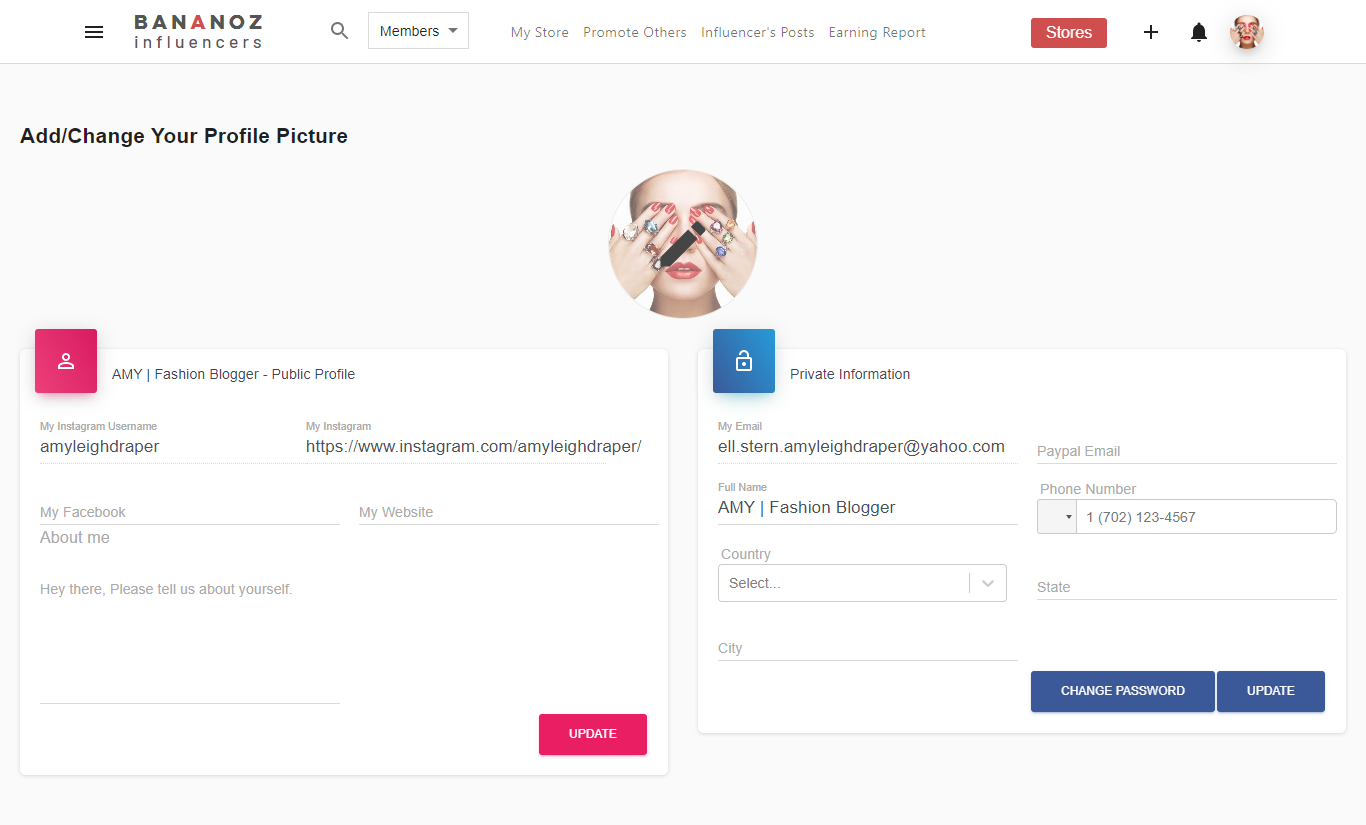
\includegraphics[height=9cm,width=14cm]{Admin/my-account.png}
\end{center}

\pagebreak

% This section type your project contents 


\textbf{Home Page -Influencer}
\begin{center}
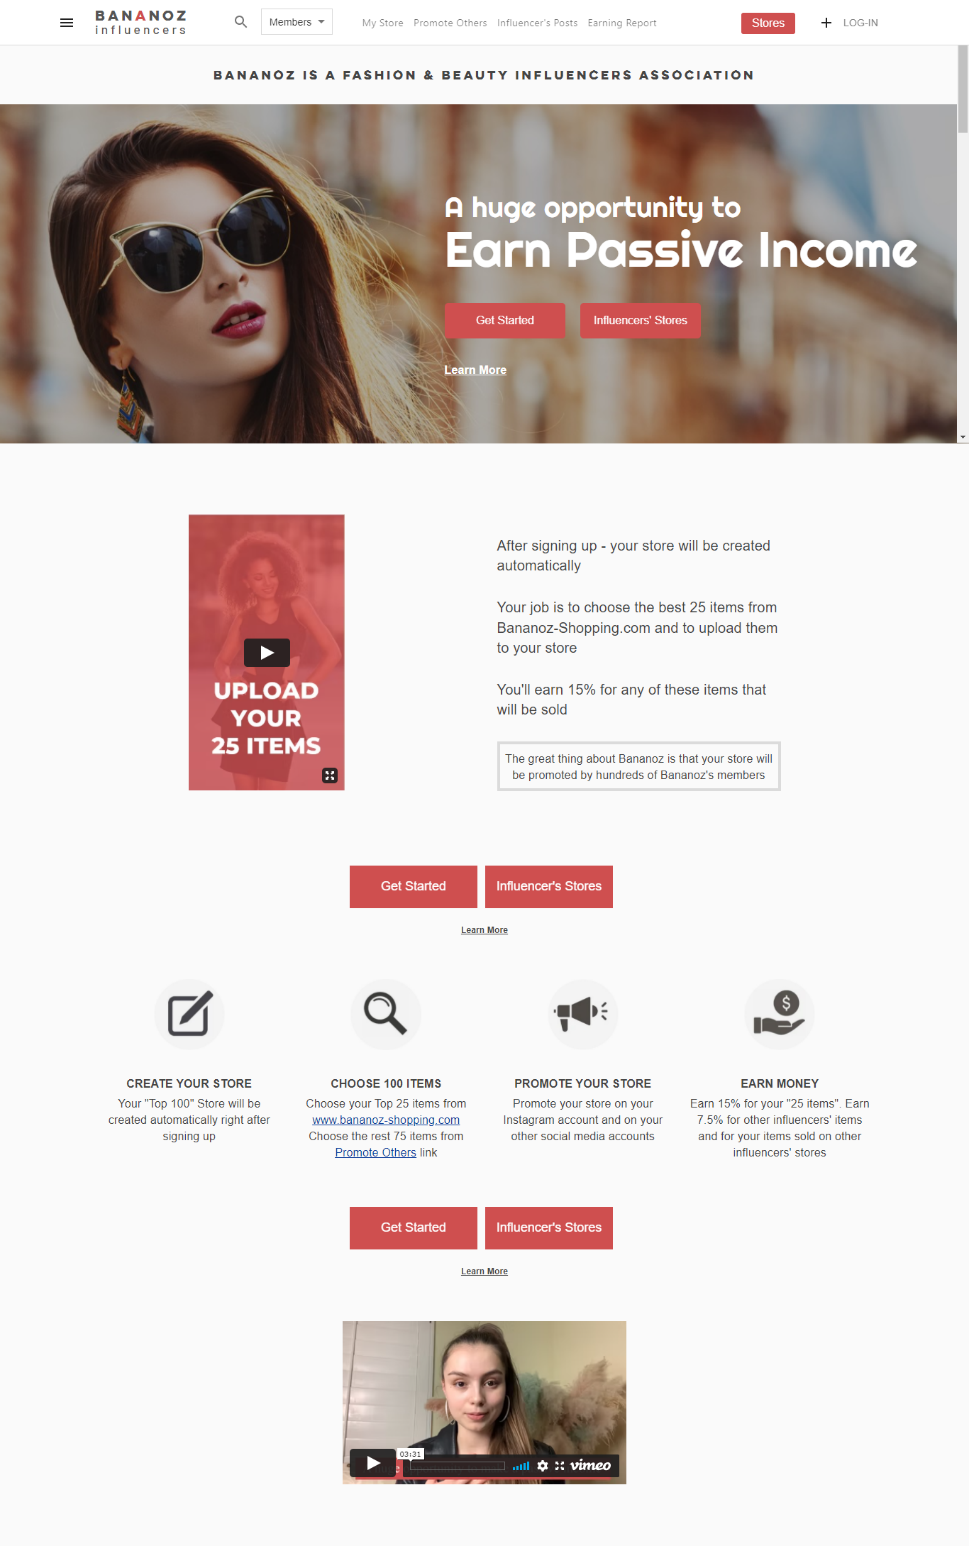
\includegraphics[height=16cm,width=14cm]{Admin/home-influencer.png}
\end{center}
\pagebreak

\pagebreak
\textbf{My Store Page}
\begin{center}
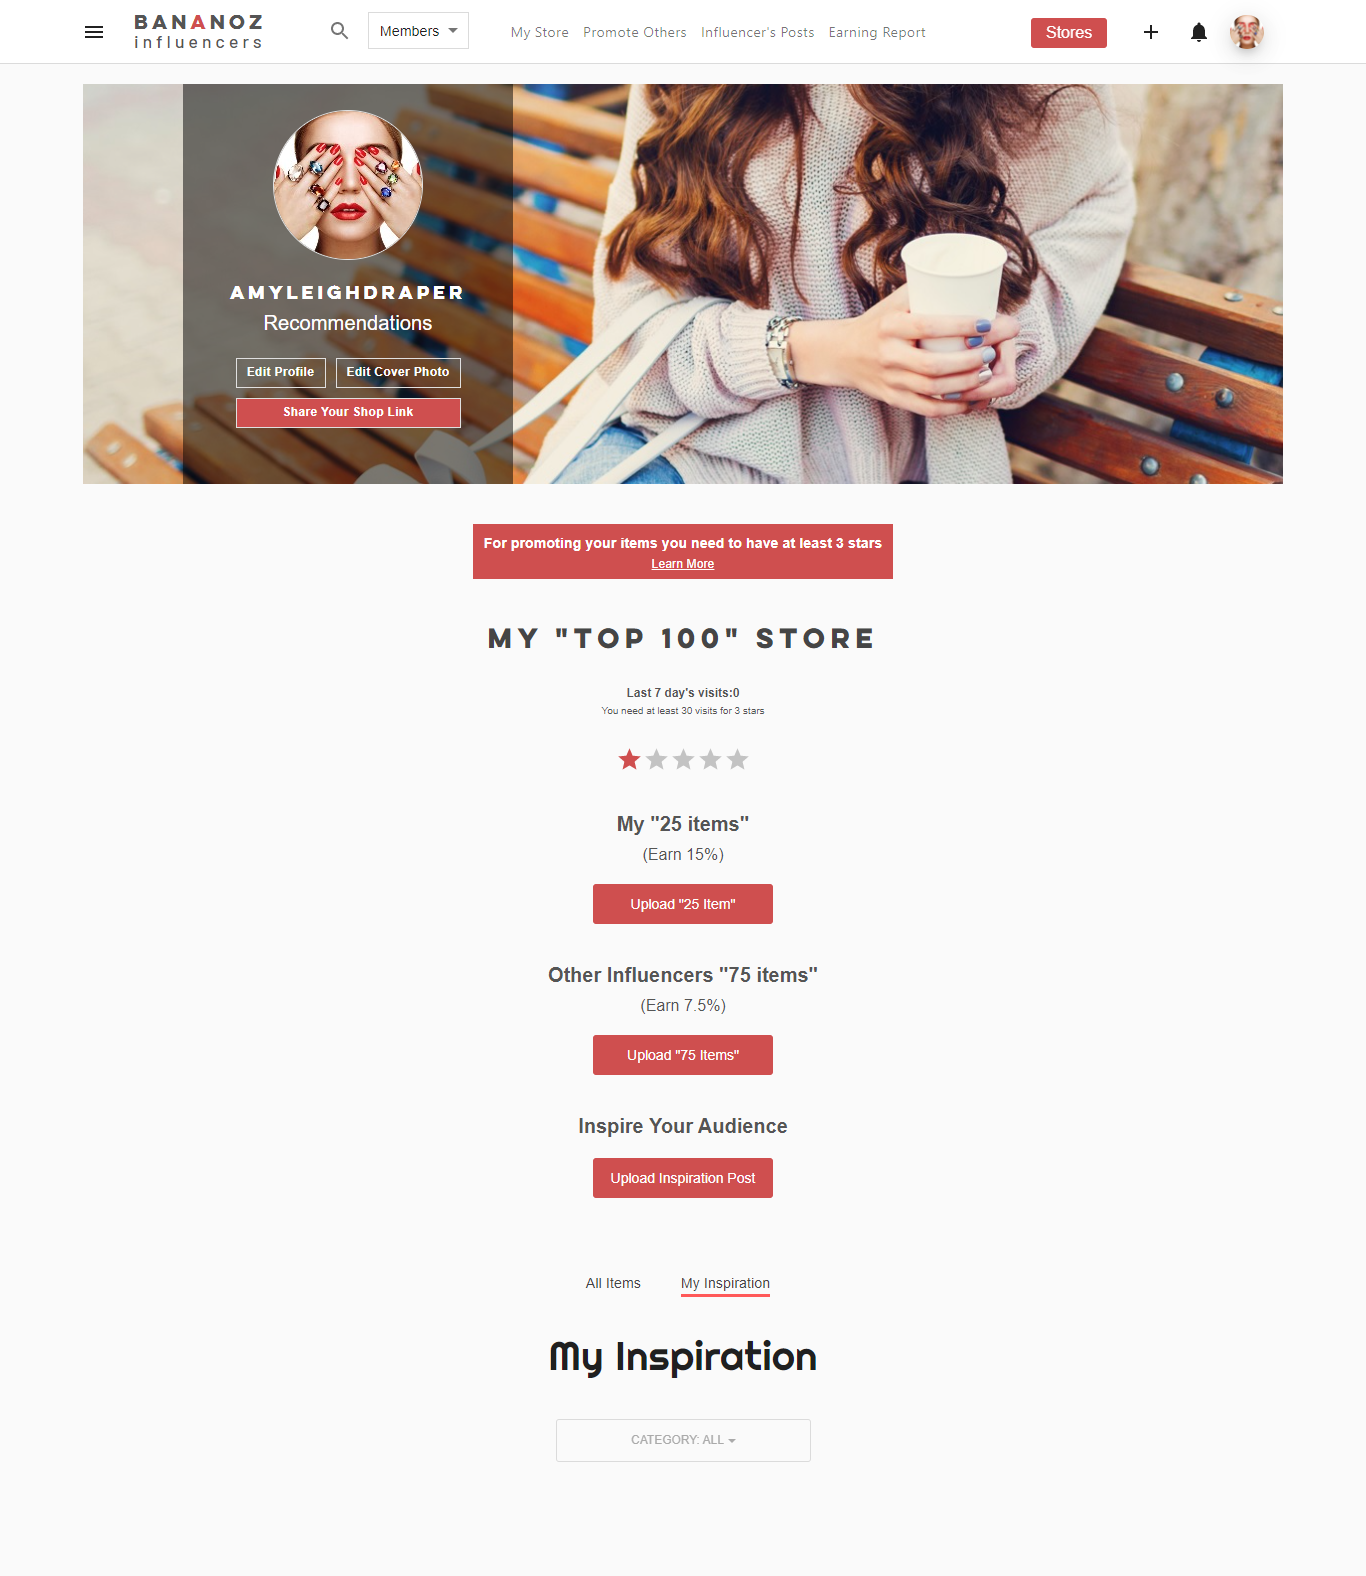
\includegraphics[height=16cm,width=14cm]{Admin/my-store.png}
\end{center}

\pagebreak


\pagebreak

\pagebreak
\textbf{Influencer’s Posts Page}
\begin{center}
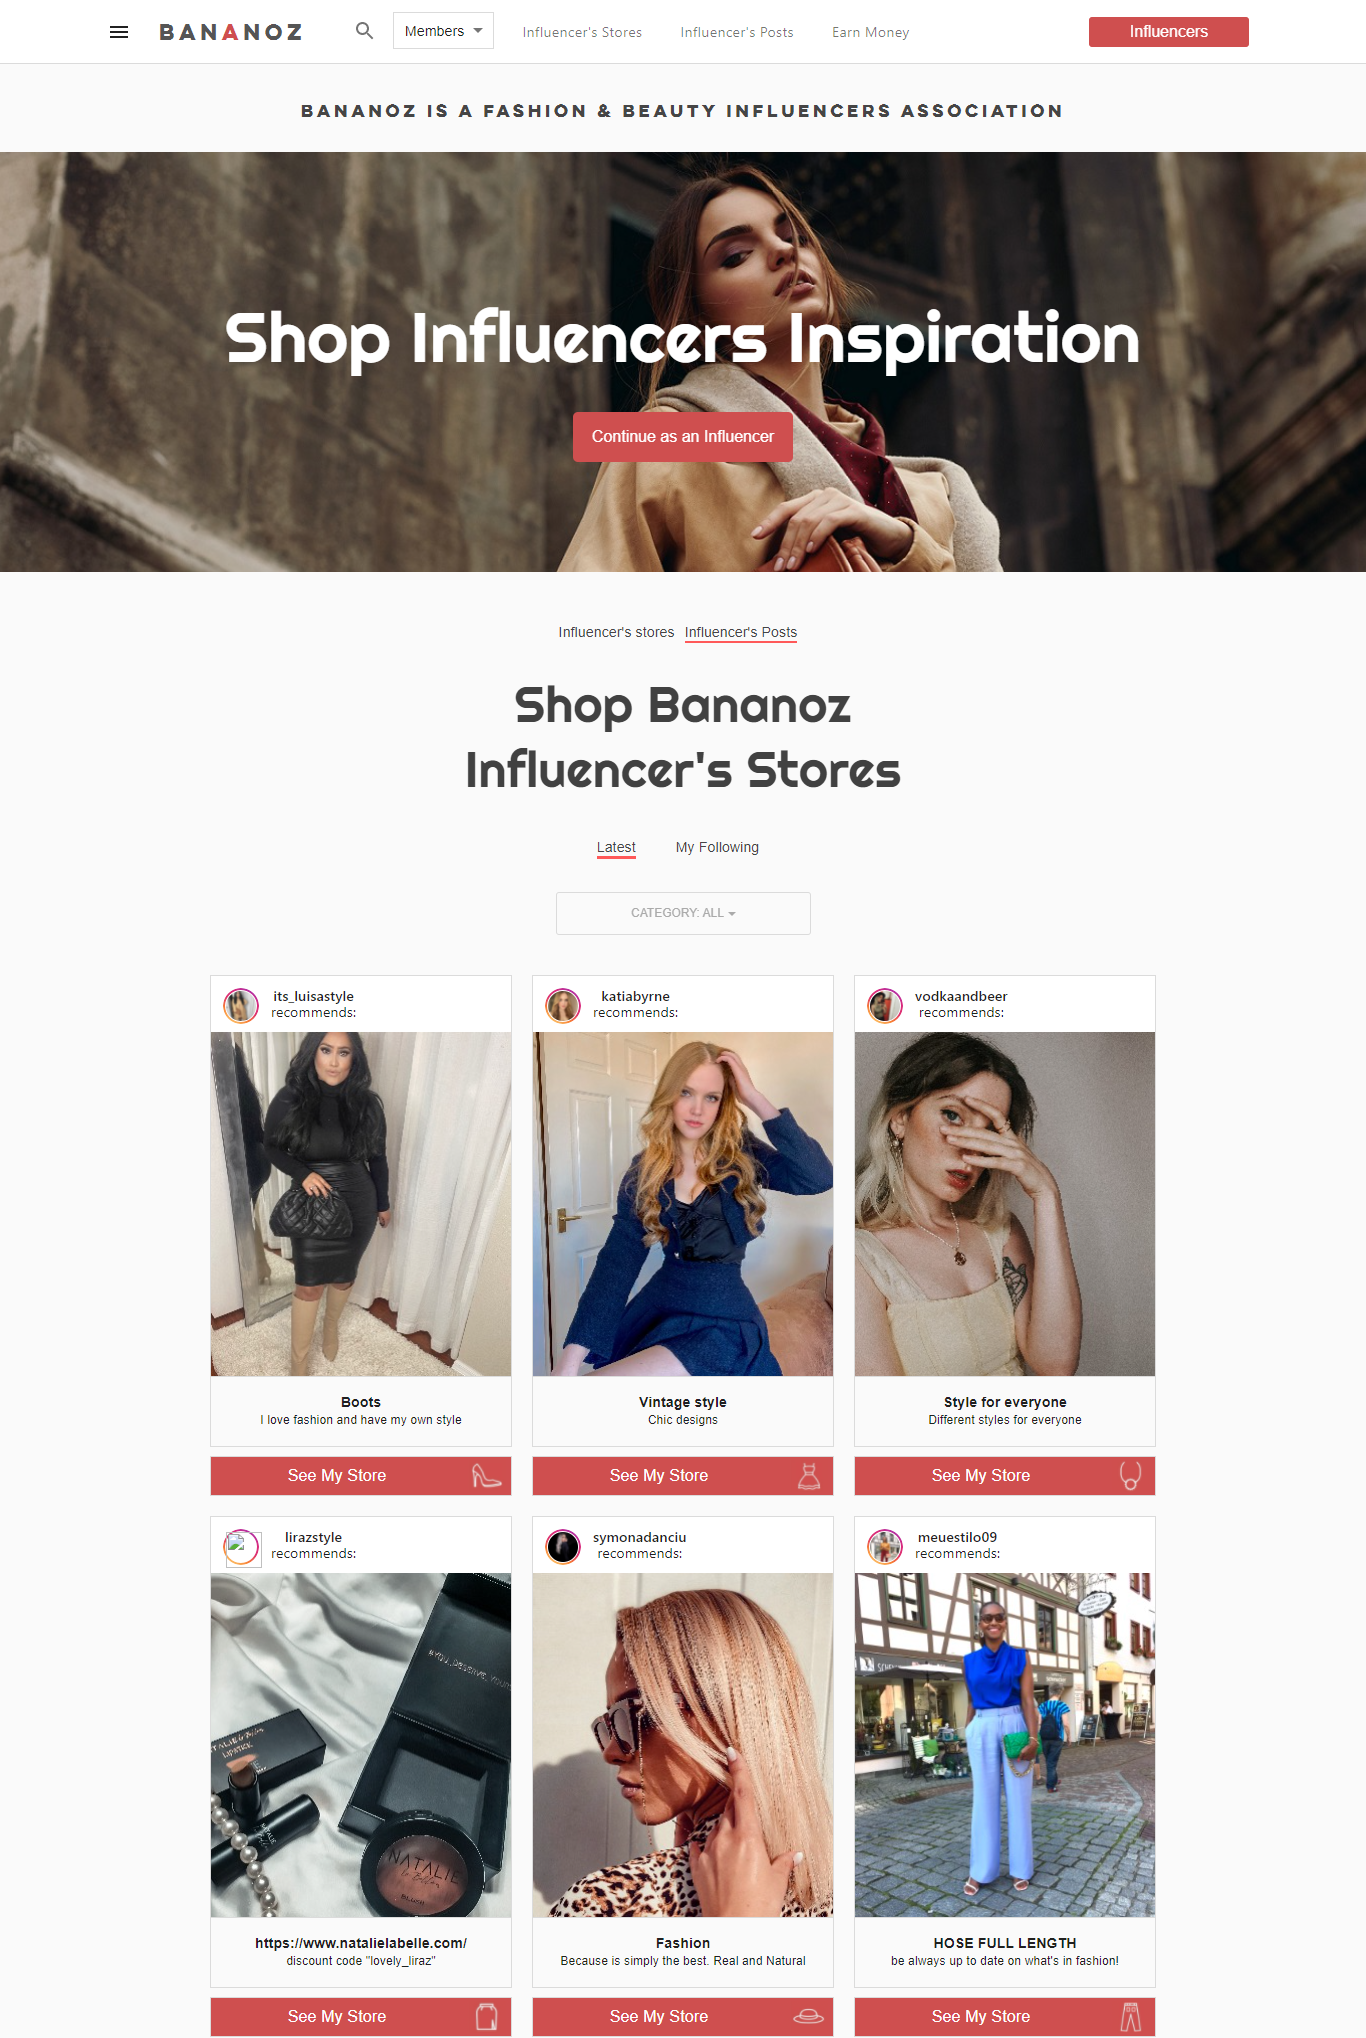
\includegraphics[height=16cm,width=14cm]{Admin/influ-post.png}
\end{center}

\pagebreak

		
		% This section type your project contents 
		

\section{Database structure}
\textbf{User:}  This table stores user details like id, username, name, password...\nolinebreak
\begin{table}[hp]
\centering

\begin{tabular}{|c|c|c|c|}
\hline
\textbf{Field Name}  & \textbf{Data Type}  & \textbf{size} &\textbf{Constraints}  \\
\hline
\_id & int & - & Primary Key,auto\_increment \\
\hline
Username &	varchar &	200 & Unique, NOT NULL.\\
\hline
First\_name & varchar &	255 & NOT NULL.\\
\hline
Access\_level & varchar & 11 &	NOT NULL\\
\hline
Email &	varchar & 60 &	Unique, NOT NULL.\\
\hline
Link &	varchar & 300 &	Unique, NOT NULL.\\
\hline
IG\_Access\_Token & varchar & 20 & Unique, NOT NULL.\\
\hline
IG\_Account\_Type & varchar & 100 & NOT NULL. \\
\hline
IG\_Followe & number & 100 & NOT NULL. \\
\hline
IG\_Followers & number & 100 & NOT NULL. \\
\hline
Image\_URL & varchar & 200 & Unique, NOT NULL. \\
\hline
Image\_URL\_HD & varchar & 200 & Unique, NOT NULL. \\
\hline
Password & varchar &	25 & NOT NULL. \\
\hline
Password\_Recovery & varchar & 15 & NOT NULL. \\
\hline
Payment & number & 20 & NOT NULL. \\
\hline
Phone\_no & number &	10 & NOT NULL. \\
\hline
Posts & blob & - & NOT NULL. \\
\hline
Created & varchar & 50 & NOT NULL. \\
\hline
Validated & varchar & 50 & NOT NULL. \\
\hline
Validated\_Token & varchar &	100 & NOT NULL. \\
\hline
Blocked & int &	- & NOT NULL. \\
\hline
Approve & int &	- & NOT NULL. \\
\hline
City & varchar &	80 & NOT NULL. \\
\hline
Country & varchar & 80 & Default, NOT NULL. \\
\hline
Last\_Posted & blob &	- & NOT NULL. \\
\hline
Last\_Promote\_Id & varchar & 30 & NOT NULL. \\
\hline
Last\_Promoted & varchar & 30 & NOT NULL. \\
\hline
Last\_Promotes & varchar & 30 & NOT NULL. \\
\hline
Max\_Promotes & int & - & NOT NULL. \\
\hline
IG\_Promotion\_Credits & int & - & NOT NULL. \\
\hline
\end{tabular}
\caption{ User}
\end{table}
\\
\\
\\
\\
\\
\textbf{Product:} This table stores Details of products and Status of product.\nolinebreak
\begin{table}[hp]
\centering
\begin{tabular}{|c|c|c|c|}
\hline
\textbf{Field Name}  & \textbf{Data Type}  & \textbf{size} &\textbf{Constraints}  \\
\hline
\_id & bigint &	20 & Foreign Key\\
\hline
Product\_Id & int & - & Primary Key,auto\_increment\\
\hline
Product\_Title &	varchar & 20 & NOT NULL \\
\hline
Product\_body &	varchar & 20  & NOTNULL \\
\hline
Product\_Vendor & varchar & 20 & NOT NULL\\
\hline
Product\_type &	varchar & 20 & NOT NULL\\
\hline
Product\_Handle &	varchar & 20 & NOT NULL\\
\hline
Product\_Image &	blob & - & NOT NULL\\
\hline
Product\_Options &	varchar & 100 & NOT NULL\\
\hline
Product\_Tags &	varchar & 100 & NOT NULL\\
\hline
created & tinyint & - & NOT NULL\\
\hline
Archive & tinyint & - & NOT NULL\\
\hline
Email &	varchar & 200 & NOT NULL\\
\hline
Username &	varchar & 80 & Unique, NOT NULL\\
\hline
Owner\_id &	varchar & 20 & Foreign Key, NOT NULL\\
\hline
Category &	varchar & 100 & NOT NULL\\
\hline
Archive &	varchar & 50 & NOT NULL\\
\hline
Last\_Update &	date & - & NOT NULL\\
\hline
Blocked &	int & - & NOT NULL\\
\hline
Is\_Promoted & int & - & NOT NULL\\
\hline
Is\_Deleted & int & - & NOT NULL\\
\hline
Product\_Variants &	varchar & 50 & NOT NULL\\
\hline
Approve &	tinyint & - & NOT NULL\\
\hline
\end{tabular}
\caption{Product}
\end{table}

\textbf{Following:} This table stores the following details.\nolinebreak
\begin{table}[hp]
\centering
\begin{tabular}{|c|c|c|c|}
\hline
\textbf{Field Name}  & \textbf{Data Type}  & \textbf{size} &\textbf{Constraints}  \\
\hline
\_id &	int & - &  Primary Key,auto\_increment \\\hline
Followee\_id &	int & - & NOT NULL \\\hline
Created & date &	- & NOT NULL \\\hline
Follower\_id & int &	- & NOT NULL \\\hline

\end{tabular}
\caption{Following}
\end{table}

\pagebreak
\textbf{Payments:}  This table stores all Payment details which are made by customers.\nolinebreak

\begin{table}[hp]
\centering
\begin{tabular}{|c|c|c|c|}
\hline
\textbf{Field Name}  & \textbf{Data Type}  & \textbf{size} &\textbf{Constraints}  \\
\hline
\_id & int &	 - & Primary Key,auto\_increment\\
\hline
Created &	date & - & NOT NULL\\
\hline
Updated\_at & date &	- & NOT NULL\\
\hline
Amount &	 number & 20 & NOT NULL\\
\hline
Beneficiary\_User & varchar & 20 & NOT NULL\\
\hline
Beneficiary\_Email & varchar & 100 & NOT NULL\\
\hline
Is\_Deleted & tinyint & - & \\
\hline
\end{tabular}
\caption{Payments}
\end{table}

\textbf{Shops:} This table stores the details of Shops.\nolinebreak
\begin{table}[hp]
\centering
\begin{tabular}{|c|c|c|c|}
\hline
\textbf{Field Name}  & \textbf{Data Type}  & \textbf{size} &\textbf{Constraints}  \\
\hline
\_id &	int	 & 11 & Primary Key,auto\_increment \\\hline
domain &	varchar & 50 & NOT NULL \\\hline
Created	 & date & - & NOT NULL \\\hline
description & varchar & 100 & NOT NULL \\\hline
is\_allowed & tinyint &  & NOT NULL \\\hline
Name & varchar &	30 & NOT NULL \\\hline
 
\end{tabular}
\caption{Shops}
\end{table}



\textbf{Messages:} This table stores the Massages.\nolinebreak
\begin{table}[hp]
\centering
\begin{tabular}{|c|c|c|c|}
\hline
\textbf{Field Name}  & \textbf{Data Type}  & \textbf{size} &\textbf{Constraints}  \\
\hline
from\_Username &	varchar &	50 &  Primary Key,auto\_increment \\\hline
to\_Username & varchar &	50 & Unique, NOT NULL \\\hline
Created  & date & - & NOT NULL \\\hline
read & varchar &	200 & NOT NULL \\\hline
Message & varchar &	200 & NOT NULL \\\hline

\end{tabular}
\caption{Messages}
\end{table}

\pagebreak


\textbf{Posts: } This table stores the details of Post's which are made by user.\nolinebreak
\begin{table}[hp]
\centering
\begin{tabular}{|c|c|c|c|}
\hline
\textbf{Field Name}  & \textbf{Data Type}  & \textbf{size} &\textbf{Constraints}  \\
\hline
\_id &	bigint &	 - & Primary Key,auto\_increment \\\hline
Link &	 varchar &	100 & Unique, NOT NULL \\\hline
Archive	 & varchar &	10 & NOT NULL \\\hline
Blocked &	bigint &	 - & NOT NULL \\\hline
Catagory &	varchar & 50 & NOT NULL \\\hline
Coin\_earned &	number &	 20 & NOT NULL \\\hline
Coin\_Invested &	number &	 20 & NOT NULL \\\hline
Coin\_Spent &	number &	 20 & NOT NULL \\\hline
Created &	date &	- & NOT NULL \\\hline
Credits\_earned &	number &	20 & NOT NULL \\\hline
Monetized\_Link &	varchar & 20 & Unique, NOT NULL \\\hline
IG\_Promoters &	int & - & NOT NULL \\\hline
Email &	varchar &	20 & Unique, Unique, NOT NULL \\\hline
Exposure &	varchar &	20 & NOT NULL \\\hline
Is\_Promoted &	tinyint & - & NOT NULL \\\hline
Last\_Update &	date & - & NOT NULL \\\hline
Likes &	int & - & NOT NULL \\\hline
Owner\_Id &	varchar & 100 & Foreign Key, NOT NULL \\\hline
Promote &	varchar & 20 & NOT NULL \\\hline
Promoting &	varchar & 20 & NOT NULL \\\hline
Shop &	varchar &	20 & NOT NULL \\\hline
Username &	varchar & 20 & Unique, NOT NULL \\\hline
Views &	varchar &	20 & NOT NULL \\\hline
Votes &	int & - & NOT NULL \\\hline
Total\_Votes &	bigint &	 - & NOT NULL \\\hline
\end{tabular}
\caption{Posts}
\end{table}\\

\pagebreak

\textbf{Promoting: } This table stores the promotion.\nolinebreak
\begin{table}[hp]
\centering
\begin{tabular}{|c|c|c|c|}
\hline
\textbf{Field Name}  & \textbf{Data Type}  & \textbf{size} &\textbf{Constraints}  \\
\hline
\_id &	int & - & Primary Key,auto\_increment \\\hline
Promoter\_post\_Id &	 int & - & Foreign Key, NOT NULL \\\hline
Promoter\_user\_Id &	int & - & Foreign Key, NOT NULL \\\hline
Promote\_User\_Id &	int & - & Foreign Key, NOT NULL \\\hline
Promote\_post\_Id &	int & - & Foreign Key, NOT NULL \\\hline
Created & date &	 - & NOT NULL \\\hline
Category & varchar &	- & NOT NULL \\\hline
Approve & tinyint &	- & NOT NULL \\\hline
 
\end{tabular}
\caption{Promoting}
\end{table}

\textbf{Product\_Promoting:} This table stores the  promotion details of product.\nolinebreak
\begin{table}[hp]
\centering
\begin{tabular}{|c|c|c|c|}
\hline
\textbf{Field Name}  & \textbf{Data Type}  & \textbf{size} &\textbf{Constraints}  \\
\hline
\_id	& int &	- & Primary Key,auto\_increment \\\hline
Promote\_product &	varchar	 & 20 & NOT NULL \\\hline
Product\_user\_Id &	 int &	- & Foreign Key, NOT NULL \\\hline
Approve & tinyint &	- & NOT NULL \\\hline
Category & varchar &	- & NOT NULL \\\hline
Created & date &	 - & NOT NULL \\\hline
Is\_Deleted & tinyint & - & NOT NULL \\\hline
Promote\_Id & int & - & Foreign Key, NOT NULL \\\hline
 
\end{tabular}
\caption{Product\_Promoting}
\end{table}

\pagebreak


\textbf{Commission:} This table stores the Commission details which are gives on products.\nolinebreak
\begin{table}[hp]
\centering
\begin{tabular}{|c|c|c|c|}
\hline
\textbf{Field Name}  & \textbf{Data Type}  & \textbf{size} &\textbf{Constraints}  \\
\hline
 \_id &	int &	11 & Primary Key,auto\_increment \\\hline
Created & date &	3 & NOT NULL \\\hline
Updated\_At & datetime &	- & NOT NULL \\\hline
User\_Id &	int & - & Foreign Key, NOT NULL \\\hline
Username &	varchar & 50 & Unique, NOT NULL \\\hline
Email &	varchar & 100 & NOT NULL \\\hline
Beneficiary\_User &	varchar & 100 & NOT NULL \\\hline
Product\_Owner\_Id &	int & - & NOT NULL \\\hline
Profile\_Owner\_Id &	int	 & - & NOT NULL \\\hline
Purchased\_At &	datetime & - & NOT NULL \\\hline
Order\_Id &	int & - & Foreign Key, NOT NULL \\\hline
Product\_id &	int & - & Foreign Key, NOT NULL \\\hline
Taxes &	number & 20 & NOT NULL \\\hline
Shipping\_Charge & number &	20 & NOT NULL \\\hline
Order\_No &	int & - & Unique, NOT NULL \\\hline
Order\_Status\_URL  & varchar &	20 & NOT NULL \\\hline
Variant\_id & int & - & NOT NULL \\\hline
Product\_title &	varchar & 50 & NOT NULL \\\hline
Link &	varchar & 200 & Unique, NOT NULL \\\hline
Product\_Price &	number &	20 & NOT NULL \\\hline
Commission\_Share &	number &	 10 & NOT NULL \\\hline
Commission\_Amount &	number &	 10 & NOT NULL \\\hline
Ownership &	varchar & 20 & NOT NULL \\\hline
Status &	tinyint & - & NOT NULL \\\hline
Is\_deleted &	tinyint & - & NOT NULL \\\hline
Is\_Promoted &	tinyint & - & NOT NULL \\\hline
Commission\_request & int & - & NOT NULL \\\hline

\end{tabular}
\caption{Commission}
\end{table}

\pagebreak

\textbf{Errors:} This table stores the errors detail.\nolinebreak
\begin{table}[hp]
\centering
\begin{tabular}{|c|c|c|c|}
\hline
\textbf{Field Name}  & \textbf{Data Type}  & \textbf{size} &\textbf{Constraints}  \\
\hline
\_id &	int & - & Primary Key,auto\_increment \\\hline
Error\_id &	int & - & NOT NULL \\\hline
Filename &	varchar & 30 & NOT NULL \\\hline
Lineno &	int & - & NOT NULL \\\hline
Line &	varchar & 10 & NOT NULL \\\hline
Name &	varchar & 20 & NOT NULL \\\hline
Type & varchar	& 20 & NOT NULL \\\hline
Error & varchar & 50 & NOT NULL \\\hline
Details &	varchar &	250 & NOT NULL \\\hline
Count &	int &	- & NOT NULL \\\hline
Created &	date &	- & NOT NULL \\\hline
Last\_occurrence &	date &	- & NOT NULL \\\hline
\end{tabular}
\caption{Errors}
\end{table}

\textbf{Sponsored\_Post} This table stores the Sponsored post details.\nolinebreak
\begin{table}[hp]
\centering
\begin{tabular}{|c|c|c|c|}
\hline
\textbf{Field Name}  & \textbf{Data Type}  & \textbf{size} &\textbf{Constraints}  \\
\hline
\_id &	int &	- & Primary Key,auto\_increment \\\hline
Owner\_id  &	int &	- & Foreign Key, NOT NULL \\\hline
Store\_id &	int &	- & Foreign Key, NOT NULL \\\hline
Description &	 varchar &	250 & NOT NULL \\\hline
Views &	int &	- & NOT NULL \\\hline
Created &	date &	- & NOT NULL \\\hline
Category &	varchar &	30 & NOT NULL \\\hline
Approve &	tinyint &	- & NOT NULL \\\hline
Image\_Link &	varchar &	250 & Unique, NOT NULL \\\hline
Monotized\_Link&	varchar &	250 & Unique, NOT NULL \\\hline
Shop\_Link &	varchar &	250 & Unique, NOT NULL \\\hline
Post\_Link &	varchar &	250 & Unique, NOT NULL \\\hline
Ad\_Link &	varchar & 250 & Unique, NOT NULL \\\hline
Fetches &	datetime &	- & NOT NULL \\\hline
Clicks &	datetime &	- & NOT NULL \\\hline
\end{tabular}
\caption{Sponsored\_Post}
\end{table}


